\documentclass{article}
\usepackage{graphicx}

\title{Assignment 7}

\date{08/11/2016}
\author{Lucas Franceschino}


\begin{document}
	\maketitle

	\section{Remarks}
		\subsection{Screenshots}
			I took some screenshots, which are in the $Screenshots$ directory.
		\subsection{Event handling}
			To handle client events on SVG image, I use list of tuple (Integer, Function). The integer represent a specific action, while Function represent the actual action. The implementation is in $Object.DrawObject$.
		\subsection{Adding sections and points in designer mode}
			When you add an element in the designer view, it look for a free emplacement automatically. ($findEmptyLocation$ in $TrainGui.TrackDesigner$)
	\section{Description of modules}
		\subsection{Directory Objects}
			\paragraph{} This directory contains modules related to $Elements$ ($Section$ and $Point$) or $Train$ and how to draw them.
			\subsubsection{Module DrawObject}
				\paragraph{} It define a class $DrawableObject$. Also, it define a function $drawObjects$ working for any $DrawableObject$.
			\subsubsection{Module Element}
				\paragraph{} An $Element$ is an instance of $DrawableObject$ and can either be a $Section$ or a $Point$. It has a label, a position and other specific things. This module define structures for $Element$, $Section$, $Point$, and define few functions to manipulate any $Element$.
				\paragraph{Choice for $Section$}
					A section has zero, one, or two signals (using two Maybe Bool fields).
				\paragraph{Choice for $Point$}
					A $Point$ has an orientation, it can be either north west or north east: either it is a line connecting a left section to an north west other section, either it is a line connecting a right section to a north east other.
					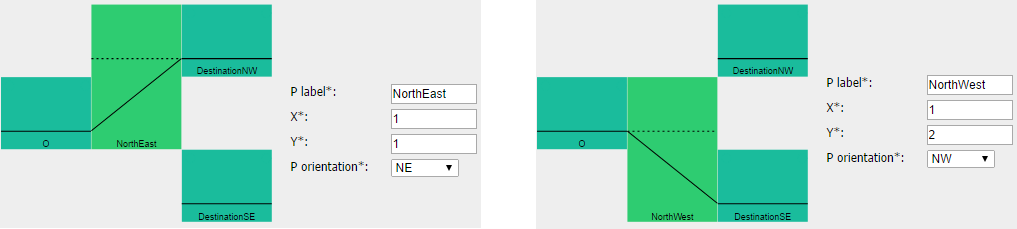
\includegraphics[width=12cm]{Point.png}
			\subsubsection{Module Train}
				\paragraph{} An $Train$ is an instance of $DrawableObject$. A train has a state (not moving, moving, destroyed) and a direction (left or right).
		\subsection{Directory TrainGui}
			\paragraph{} This directory contains modules to handle how is drawn the GUI for each roles.
			\subsubsection{Module ChooseRole}
			\subsubsection{Module DriveTrain}
			\subsubsection{Module TrackController}
			\subsubsection{Module TrackDesigner}
			\subsubsection{Module MakeTrainMove}
				This module watch the time to animate trains movements if necessary. It provide a function $makeTrainMove$ looping on watching time. If no any train moves, then it stops looping, and when a train driver will put his train in motion, the $makeTrainMove$ function is called again.

				To prevent multiple instance of $makeTrainMove$, a shared boolean value $resetAreTrainsMoving$ is used.

				This function also detects trains collisions and train out of rails.
		\subsection{Module GlobalVisualStyle}
			Define visual style of SVG drawn objects.
		\subsection{Module State}
		\subsection{Module ImageTask}
			This module is the bridge from $TrainGui$ modules to $Objects$ ones. Indeed, $ImageTask$ is the task generating images.
		\subsection{Module RailwayGame}
			It is the main module, which directly launch $chooseRole$ routine.




		There is two main directories: $Objects$ and $TrainGui$.
\end{document}